\chapter{Mapeamento objeto-relacional (ORM)}\label{cap:cap3}

\begin{flushright}
	\textit{
		É melhor você tentar algo, vê-lo não funcionar \\ e aprender com isso, do que não fazer nada.
	} \\
	
	\textbf{Mark Zuckerberg}
\end{flushright}

Criar um banco de dados, ou mais formalmente o Sistema Gerenciador de Banco de Dados (SGBD), é uma tarefa complexa presente em todos os projetos. Escolher qual será utilizar em meio a tantos como: my\textbf{sql, sqlserver, oracle, sqlite , postgre, mongodb e etc}, ou, qual se adapta melhor ao projeto é uma decisão que deve ser tomada com cautela.

Outro fato é a forma com que os dados são tratados em cada um. Por exemplo, para um campo \textbf{id} que deve ser auto-incrementado, no Postgres usando o seguinte código SQL:

\begin{minted}[frame=single,framesep=10pt,breaklines,linenos,tabsize=2,autogobble]{sql}
	CREATE TABLE Pessoas (
		id SERIAL NOT NULL,
		nome varchar
	);
\end{minted}

Já no Mysql, o mesmo código seria escrito da seguinte forma:

\begin{minted}[frame=single,framesep=10pt,breaklines,linenos,tabsize=2,autogobble]{javascript}
	CREATE TABLE Pessoas (
		id int NOT NULL AUTO_INCREMENT,
		nome varchar
	);
\end{minted}

Logo, caso houvesse uma mudança, nosso código teria que ser alterado para satisfazer a nova base de dados com todas as suas diferenças. Assim, pensando nas possíveis mudanças que o projeto pode ter durante sua vida útil, foram desenvolvidas algumas técnicas para facilitar a vida dos desenvolvedores. Uma que iremos comentar é o Object Relational Mapping (ORM) ou Mapeamento Objeto Relacional. Para diminuir a complexidade, já que o ORM torna o banco de dados mais próximo da arquitetura de classe, removendo os comando SQL de vista, para que possamos focar em ``Qual é o fluxo que minha aplicação deve seguir'' e deixando de lado ``Qual é a query que eu deveria usar aqui?''. Então, nesse aspecto, iremos abordar um pouco sobre o que são ORM, suas práticas e exemplos usando JavaScript.

\section{ORM: o que é? }

Como já citei anteriormente um ORM é a siga em inglês para Mapeamento Objeto Relacional e consiste em manter o uso de orientação a objetos e um pouco do conceito de non-query, pois serão raros os momentos nos quais teremos que escrever uma linha de código SQL \cite{Aylon2020Muramatsu}.Um ORM é uma solução completa para resolver a incompatibilidade de \textbf{impedância} entre objetos de programa e tabelas de banco de dados, promovendo bancos de dados relacionais com recursos de orientação a objetos \cite{song2012use}.

Outro fato muito importante e curioso sobre os ORM é que eles operam como um agente de banco de dados, sendo possível através de pouquíssimas mudanças, utilizar o mesmo código para mais de um banco de dados. Não importa se ele está em Mysql, SqlServer ou até mesmo Oracle. Ele consegue agir da mesma forma em alguns bancos de dados, você só precisa mudar o driver de conexão e está pronto para uso. Neste conceito é importante lembrar que cada uma de nossas tabelas são vistas como uma instância de uma classe, tendo suas características declaradas diretamente na sua classe ``esquema''. Quando trabalhamos com esse tipo de esquema sempre teremos um arquivo de configuração, responsável por fornecer os dados para que o componente de ORM possa se comunicar com o banco e aplicação. Uma outra questão que pode causar dúvidas é como gerar o banco de dados através dessas classes que comentamos anteriormente. Bom veremos isso na prática mais a abaixo \cite{Aylon2020Muramatsu}.

Além da manipulação, outra preocupação, quando se retrata o cenário de desenvolvimento de software com banco de dados, é a segurança. Ai utilizar um ORM (consolidado) adquirimos a possibilidade de direcionar os esforços do projeto para a inovação mantendo a confiabilidade, segurança, e tradição dos bancos de dados relacionais.

\section{ORM: como funciona?}

Para facilitar a aplicação desta técnica surgiram os frameworks ORM, como por exemplo, o Hibernate para Java, o ActiveRecord para Ruby, e o que usaremos para nossos projeto o Sequelize para NodeJS (JavaScript). Desta forma, esses frameworks se localizam em uma camada intermediária entre a lógica da sua aplicação e o seu SGDB \cite{orm202netmagazine}.

O framework passa a receber as solicitações de interação com o SGDB através de objetos de sua aplicação e gera automaticamente todo o SQL necessário para a operação solicitada, nos poupando do trabalho de escrita e manutenção deste SQL e abstraindo o uso do SGDB, fazendo com que nos preocupemos apenas com nosso modelo de objetos. Além disso, o framework já trata as variações de tipos de dados existentes entre nossa aplicação e nosso SGDB \cite{orm202netmagazine}.

\begin{figure}[H]
	\centering
	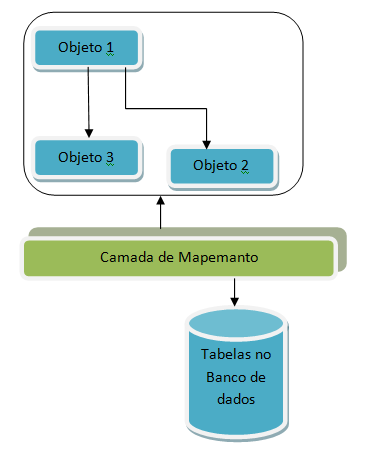
\includegraphics[scale=0.5]{imagens/orm.png}
	\caption{
		Ilustração do mapeamento
		Fonte: \cite{orm202netmagazine}
	}
	\label{fig: }
\end{figure}

O ORM funciona através do mapeamento das características da base de dados para os objetos de nossa aplicação. O primeiro conceito chave é traçar um paralelo entre Classe x Tabela e Propriedade x Coluna. O ORM nos permite informar em que tabela cada classe será persistida e em que coluna do SGDB cada propriedade ficará armazenada.

\begin{figure}[H]
	\centering
	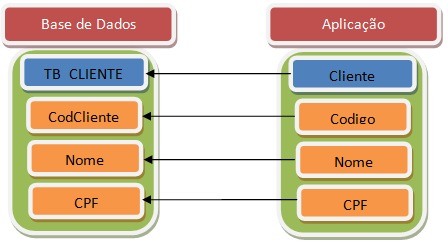
\includegraphics[scale=0.6]{imagens/mapeamentoorm.png}
	\caption{
		 Ilustração de uma classe para uma tabela
		Fonte: \cite{orm202netmagazine}
	}
	\label{fig:mapeamentoorm}
\end{figure}

\section{Configurando o frameworks ORM Sequelize}

O Sequelize possui um utilitário de linha de comando chamado \textbf{Sequelize CLI} que auxilia em diversas atividades incluindo funcionalidades para nos ajudar com \textbf{migrations}, as quais veremos mais a frente. 

De forma geral, vamos iniciar um novo projeto Node usando as instruções mais básicas. Primeiro, crie um diretório e, a partir dele, inicie um novo projeto.

\begin{minted}[frame=single,framesep=10pt,breaklines,linenos,tabsize=2,autogobble]{bash}
	mkdir novo-projeto
	cd novo-projeto
	npm init -y
\end{minted}

Logo após, ainda no diretório, adicione as bibliotecas que usaremos

\begin{minted}[frame=single,framesep=10pt,breaklines,linenos,tabsize=2,autogobble]{bash}
	npm install sequelize pg --save
	npm install --save-dev sequelize-cli
\end{minted}

Agora, vamos inicializar nosso projeto com o \textbf{Sequelize-CLI}, rodando o comando abaixo.

\begin{minted}[frame=single,framesep=10pt,breaklines,linenos,tabsize=2,autogobble]{bash}
	npx sequelize-cli init
\end{minted}

O resultado será o retorno e a criação de alguns diretórios listados abaixo.

\begin{minted}[frame=single,framesep=10pt,breaklines,linenos,tabsize=2,autogobble]{bash}
Created "config/config.json"
Successfully created models folder at ...
Successfully created migrations folder at ...
Successfully created seeders folder at ...
\end{minted}

O diretório \textbf{Models} nós já conhecemos. Contudo, os novos criados tem como função conectar ao banco e criar tabelas e adicionar dados. Vamos ver cada um:

\begin{itemize}
	\item \textbf{config/config.json} é o local onde colocaremos os dados para conexão, como usuário, senha, host, etc. Nesse arquivo, um dos parâmetros é o \textbf{dialect}. Nele devemos colocar o SGBD desejado. Por padrão, ele é gerado como \textbf{mysql}, por isso, vamos mudar para \textbf{postgres}/
	\item \textbf{migrations} é o local no qual criaremos nosso código equivalente ao SQL para a criação das tabelas, porém, usando apenas JavaScript.
	\item \textbf{seeders} será onde criaremos o código que semeará os dados no banco.
\end{itemize} 

\section{Criando nosso primeiro modelo e migração}

Vamos criar um cenário bem simples no qual criaremos uma nova tabela no banco de dados, Para criar uma \textbf{migration}, podemos usa o seguinte comando no console, que baixa e executa o \textbf{Sequelize CLI} com o comando de criação de migration.

\begin{minted}[frame=single,framesep=10pt,breaklines,linenos,tabsize=2,autogobble]{bash}
	npx sequelize-cli model:create --name usuario --attributes nome:string
\end{minted}

O comando acima irá criar uma pasta \textbf{migrations} no seu projeto (se ela não existir) e dentro dela nosso primeiro arquivo de \textbf{migration}, idêntico ao abaixo.

\begin{minted}[frame=single,framesep=10pt,breaklines,linenos,tabsize=2,autogobble]{javascript}
	'use strict';
	module.exports = {
		async up(queryInterface, Sequelize) {
			await queryInterface.createTable('usuarios', {
				id: {
					allowNull: false,
					autoIncrement: true,
					primaryKey: true,
					type: Sequelize.INTEGER
				},
				nome: {
					type: Sequelize.STRING
				},
				createdAt: {
					allowNull: false,
					type: Sequelize.DATE
				},
				updatedAt: {
					allowNull: false,
					type: Sequelize.DATE
				}
			});
		},
		async down(queryInterface, Sequelize) {
			await queryInterface.dropTable('usuarios');
		}
	};
\end{minted}

Toda migração possui um \textbf{up} e um \textbf{down}, referente ao script de migration (criação) e o rollback (desfaz o que foi criado) da mesma. Isso permite que em caso de necessidade seja desfeita a migration, permitindo a gestão das alterações do banco de dados com muito mais detalhe.

Também será criado um modelo com o código abaixo

\begin{minted}[frame=single,framesep=10pt,breaklines,linenos,tabsize=2,autogobble]{javascript}
	'use strict';
	const { Model } = require('sequelize');
	module.exports = (sequelize, DataTypes) => {
		class usuario extends Model {
			/**
			* Helper method for defining associations.
			* This method is not a part of Sequelize lifecycle.
			* The `models/index` file will call this method automatically.
			*/
			static associate(models) {
				// define association here
			}
		}
		usuario.init({
			nome: DataTypes.STRING
		}, {
			sequelize,
			modelName: 'usuario',
		});
		return usuario;
	};
\end{minted}

Assim, para enviar os dados ao banco, devemos executar dois comandos, o primeiro para criar o banco e outro para criar as tabelas do banco selecionado.

\begin{minted}[frame=single,framesep=10pt,breaklines,linenos,tabsize=2,autogobble]{javascript}
	npx sequelize-cli db:create // Não deve ser usado para o ElephantSQL
	npx sequelize-cli db:migrate
\end{minted}

\section{Adicionado o Frameworks Express ao Projeto}

Para que possamos utilizar os recursos do \textbf{sequelize} em um ambiente web, vamos usar no frameworks \textbf{ExpressJS}. Para tanto, crie um arquivo, na raiz do projeto com o nome de \textbf{index.js} e adicione o seguinte código:

\begin{minted}[frame=single,framesep=10pt,breaklines,linenos,tabsize=2,autogobble]{javascript}
	var express = require('express');
	var app = express();
	
	app.get('/', function(req, res) {
		res.send('Olá Mundo!');
	});
	
	app.listen(3000, function() {
		console.log('App de Exemplo escutando na porta 3000!');
	});
\end{minted}

Vamos adicionar o ExpresssJS ao nosso projeto executando o código abaixo no terminal.

\begin{minted}[frame=single,framesep=10pt,breaklines,linenos,tabsize=2,autogobble]{bash}
	npm i express --save
\end{minted}

Outra biblioteca opcional e o \textbf{nodemon} que auxilia no desenvolvimento executando o \textit{restart} da aplicação;

\begin{minted}[frame=single,framesep=10pt,breaklines,linenos,tabsize=2,autogobble]{javascript}
	npm i nodemon --save-dev 
\end{minted}

Agora, edite o arquivo \textbf{package.json} e altere a seguinte linha:

\begin{minted}[frame=single,framesep=10pt,breaklines,linenos,tabsize=2,autogobble]{javascript}
	// Tercho código antigo
	"scripts": {
		"test": "echo \"Error: no test specified\" && exit 1"
	},
\end{minted}

\begin{minted}[frame=single,framesep=10pt,breaklines,linenos,tabsize=2,autogobble]{javascript}
	// Trecho código novo
	"scripts": {
		"start": "nodemon index.js" // caso esteja usando o nodemon
	},
	
	"scripts": {
		"start": "node index.js" // caso não esteja usando o nodemon
	},
\end{minted}

Por fim, executando o `npm start` e abrindo o endereço `localhost:3000` devemos visualizar a seguinte mensagem:

\begin{figure}[H]
	\centering
	\frame{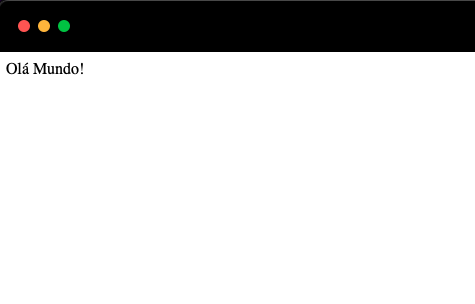
\includegraphics[scale=0.4]{imagens/olamundo.png}}
	\caption{
		Fonte: O autor
	}
	\label{fig:olamundo}
\end{figure}

Agora, se tudo deu certo, estamos prontos para criar nossas interações com o banco de dados, também conhecido como CRUD.

\section{CRUD com Sequelize}\label{sec:crudsequelize}

Os conceitos sobre CRUD (Create, Read, Update e Delete), já foram abordados no Capítulo \ref{sub:crud}. Portanto, não iremos retornar o conceitos, mas, apenas aplicá-lo.

\subsection{Inserindo dados - Create}

Agora vamos iniciar nosso CRUD com o C de Create. O Sequelize fornece alguns métodos para a inserção de dados, sendo a mais direto deles o método \textbf{create}. Esse método cria imediatamente o registro na tabela com o \textbf{objeto} passado por parâmetro. Veja o código:

\newpage

\begin{minted}[frame=single,framesep=10pt,breaklines,linenos,tabsize=2,autogobble]{javascript}
	const usuario = await Usuario.create({
		nome: 'Picolo'
	})
\end{minted}

Contudo, como estamos usando o ExpressJS, vamos adicionar o código criado em um rota com o verbo HTTP \textbf{Get} inicialmente. 

\begin{minted}[frame=single,framesep=10pt,breaklines,linenos,tabsize=2,autogobble]{javascript}
	var express = require('express');
	var { usuario } = require('./models');
	
	var app = express();
	
	app.use(express.json());
	app.use(express.urlencoded({ extended: true}));
	
	app.post('/', async function(req, res) {
		var resultado = await usuario.create()
		res.json(resultado);
	});
	
	app.listen(3000, function() {
		console.log('App de Exemplo escutando na porta 3000!');
	});
\end{minted}

Note as linhas 2. 6 e 7. Elas não existias no código anterior e foram adicionado, respectivamente, para importar o modelo \textbf{usuario} para nossas rotas e realizar parsing do conteúdo das requisições que ela receber. 

Ao rodar a aplicação agora você vai notar que no console vão aparecer algumas informações relevantes desta vez, como, por exemplo, o SQL do INSERT (porque ela não existia) que foi gerado automaticamente para você.

\begin{figure}[H]
	\centering
	\frame{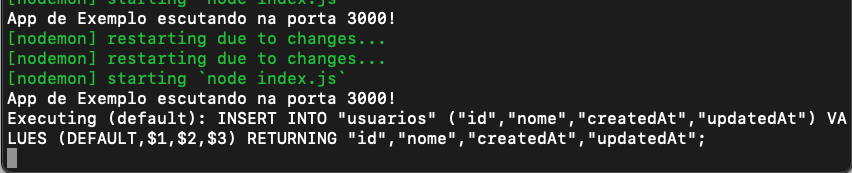
\includegraphics[scale=0.4]{imagens/resultado_create.png}}
	\caption{
		Fonte: O autor
	}
	\label{fig:resutadoinset}
\end{figure}

\subsection{Retornando dados do banco - Read}

Agora vamos fazer o R do CRUD, de Read/Retrieve. Ele é ainda mais simples do que o Create, basta usarmos a função \textbf{findAll} disponibilizada pelo nosso objeto \textbf{Usuario}, que teremos um array de produtos à nossa disposição. 

\begin{minted}[frame=single,framesep=10pt,breaklines,linenos,tabsize=2,autogobble]{javascript}
	app.get('/', async function(req, res) {
		var resultado = await usuario.findAll();
		res.json(resultado);
	});
\end{minted}

Caso seja necessário fazer uma busca no banco para retornar apenas um \textbf{usuário}, podemos utilizar o método findByPk ou findOne

\begin{minted}[frame=single,framesep=10pt,breaklines,linenos,tabsize=2,autogobble]{javascript}
	app.get('/:id', async function(req, res) {
		var resultado = await usuario.findByPk(req.params.id);
		res.json(resultado);
	});

	app.get('/:id', async function(req, res) {
		var resultado = await usuario.findOne({
			where: {
				id: req.params.id
			}
		});
		res.json(resultado);
	});
\end{minted}

Aqui vale uma explicação sobre as três propriedades de requisição que são preenchidas de diferentes formas dependendo da origem:

\textbf{req.query} vem de parâmetros de consulta na URL, como link, em que req.query.name obtem o parâmetro passado pela seguinte url `url/teste?nome=teste`

\textbf{req.params} vem de segmentos de caminho do URL que correspondem a um parâmetro na definição de rota, como /song/:id. Então, com uma rota usando essa designação e uma URL como /song/48586 , então req.params.id retornará "48586" .

Ja a  propriedade \textbf{req.body} vêm de uma postagem de formulário em que os dados do formulário (que são enviados no conteúdo do corpo) foram analisados nas propriedades da tag body.

\section{Atualizando dados - Update}

O próximo passo é atualizarmos um item da nossa tabela, o U do CRUD: Update! Para atualizarmos um item, primeiro precisamos retorná-lo do banco de dados usando alguma função de find do Sequelize. No passo anterior, usamos a findByPk para retornar o produto com ID 1. Vamos escrever o nosso código de update imediatamente abaixo.

\begin{minted}[frame=single,framesep=10pt,breaklines,linenos,tabsize=2,autogobble]{javascript}
	app.put('/:id', async function(req, res) {
		// Buscando dados
		var resultado = await usuario.findByPk(req.params.id);
		
		// Atualizada dados
		resultado.nome = req.body.nome
		var novo_resultado = await resultado.save();
		res.json(novo_resultado);
	});
\end{minted}

\section{Deletando dados - Delete}

E por fim, vamos ao D do CRUD, de DELETE! Assim como para salvar e retornar dados existem diversas formas de fazer, para o Delete não é diferente. Você pode usar Produto.destroy e passar um where por parâmetro, ou então retornar um produto e usar a função destroy do próprio objeto retornado, você decide.

\begin{minted}[frame=single,framesep=10pt,breaklines,linenos,tabsize=2,autogobble]{javascript}
	app.delete('/:id', async function(req, res) {
		var resultado = await usuario.destroy({ 
			where: { id: req.params.id }
		});
		
		res.json(resultado);
	});
\end{minted}

\section{Padrão de rotas}

Se vocês perceberam, as rotas seguem um padrão. Este pode ser usado em todos os projetos da forma descrita abaixo, sendo elas, as rotas, o básico de um projeto. Outras podem ser criadas especificadamente para atender determinada necessidade.

\begin{minted}[frame=single,framesep=10pt,breaklines,linenos,tabsize=2,autogobble]{javascript}
	app.get('/', async function(req, res) {
		// Listar todos os dados
	});
	
	app.get('/:id', async function(req, res) {
		// Listar dado específico
	});
	
	app.put('/:id', async function(req, res) {
		// Atualizar dado específico
	});
	
	app.post('/', async function(req, res) {
		// Adicionar um novo dado
	});
	
	app.delete('/:id', async function(req, res) {
		// Deletar dado específico
	});
\end{minted}

\section{Relacionamentos com Sequelize}

Ao trabalharmos com banco de dados relacionais, pela própria definição do nome, percebe-se que os relacionamentos se fazem presente. Dessa forma, o Sequelize, que é o ORM que estamos utilizando, tem mecanismos para abstrair os relacionamentos e ``importá-los'' para a programação orientada a objeto. 

\subsection{Tipos de relacionamento}

Os tipos de relacionamento em um banco relacional, provavelmente, você já conhece. Sendo eles: 

\begin{itemize}
	\item 1 para 1
	\item 1 para N
	\item N para N
\end{itemize}

O Sequelize é compatível com as associações citadas, e os métodos de criação de relacionamentos, respectivamente, são:

\begin{itemize}
	\item hasOne (tem um)
	\item belongsTo (pertence a)
	\item hasMany (tem muitos)
	\item belongsToMany (pertence a muitos)
\end{itemize}

\section{Criando o primeiro relacionamento com a entidade \textbf{Usuario}}

Utilizando a entidade \textbf{Usuario} criada anteriormente, vamos criar uma nova entidade chamada \textbf{Empresa} com apenas o atributo \textbf{nome}. 

\begin{minted}[frame=single,framesep=10pt,breaklines,linenos,tabsize=2,autogobble]{bash}
	npx sequelize-cli model:create --name empresa --attributes nome:string
\end{minted}

Agora, devemos relacionar \textbf{Empresa} com \textbf{Usuario}, no qual, as duas entidades devem possuir a seguinte relação:

\begin{figure}[H]
	\centering
	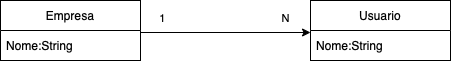
\includegraphics[scale=0.8]{imagens/empresa-usuario.png}
	\caption{
		Fonte: O Autor
	}
\end{figure}

Para tanto, devemos adicionar um novo atributo em \textbf{Usuário} que represente a \textbf{chave estrangeira} que referencia a tabela \textbf{empresas} que será gerada no banco de dados pelo Sequelize. Porém, nosso banco com a tabela \textbf{usuarios} já foi criada e, não devemos alterar as migração já persistida no banco. Para isso então, devemos criar uma  \textbf{migração} que adicione os atributos desejados, da seguinte forma:

\begin{minted}[frame=single,framesep=10pt,breaklines,linenos,tabsize=2,autogobble]{bash}
	npx sequelize-cli migration:create --name adicionar-empresa-id-para-usuario
\end{minted}

E, diferente de quanto criamos o modelo, as migrações não adicionam o código para que seja adicionado o atributo. Logo, devemos realizar as mudanças de forma manual. Abra o arquivo criado e adicione o seguinte código:

\begin{minted}[frame=single,framesep=10pt,breaklines,linenos,tabsize=2,autogobble]{javascript}
	'use strict';
	
	module.exports = {
		async up (queryInterface, Sequelize) {
			await queryInterface.addColumn('usuarios', 'empresaId', {
				allowNull: false,
				type: Sequelize.INTEGER,
				references: { model: 'empresas', key: 'id' }
			})
		},
		
		async down (queryInterface, Sequelize) {
			await queryInterface.removeColumn('pacientes', 'empresaId')
		}
	};
\end{minted}

Neste momento, você também deve criar todas as rotas necessárias para manipular os dados de uma \textbf{empresa}. Caso não lembre, recomendo que retorno a seção \ref{sec:crudsequelize}.
Assim, usando o Sequelize, a nível de Banco de Dados, criamos o relacionamento. Agora, devemos criar o mesmo usando as referências do Sequelize.

\section{Relacionamento 1 para N}

Para relacionarmos \textbf{empresa} com \textbf{usuario}, devemos usar os métodos de relacionamento presentes no Sequelize listando anteriormente. No caso de um relacionamento \textbf{1 para N} dizemos que:

\begin{itemize}
	\item \textbf{Um usuário pertence a uma empresa}
	\item \textbf{Já uma empresa, possui muitos usuários}
\end{itemize}

Adicionado ao código para cada classe do respectivo modelo, ficaria da seguinte forma:

\begin{minted}[frame=single,framesep=10pt,breaklines,linenos,tabsize=2,autogobble]{javascript}
	// Entidade Empresa
	static associate(models) {
		this.hasMany(models.usuario, { as: 'usuarios'})
	}

	// Entidade Usuario
	static associate(models) {
		this.belongsTo(models.empresa, {as: 'empresa'})
	}
\end{minted}

\subsection{Retornado dados por meio do relacionamento criado}

Agora, vamos retornar os dados de cada entidade. Um \textbf{usuário} deve estar contido dentro de uma empresa. Assim, vamos criar uma rota para retornar a empresa que o usuário está relacionado.

\begin{minted}[frame=single,framesep=10pt,breaklines,linenos,tabsize=2,autogobble]{javascript}
	app.get('/usuarios/:id/empresa', async function(req, res) {
		var resultado = await usuario.findByPk(req.params.id, {include: 'empresa'});
		res.json(resultado.empresa);
	});
\end{minted}

E da mesma forma, vamos criar uma rota que retorne todos os usuários de uma empresa.

\begin{minted}[frame=single,framesep=10pt,breaklines,linenos,tabsize=2,autogobble]{javascript}
	app.get('/empresas/:id/usuarios', async function(req, res) {
		var resultado = await empresa.findByPk(req.params.id, {include: ['usuarios']});
		res.json(resultado.usuarios);
	});
\end{minted}

\section{Exercício de fixação}

Crie dois modelos (usando o sequelize-cli) seguindo o Diagrama Entidade Relacional (DER) utilizado no trabalho do primeiro bimestre. Crie todas as rotas necessárias.

\begin{figure}[H]
	\centering
	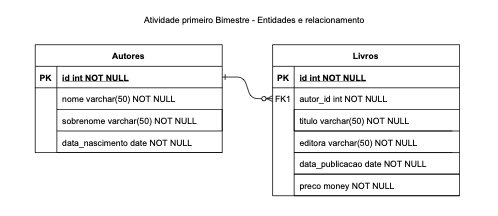
\includegraphics[scale=0.7]{imagens/der.png}
	\caption{
		Relacionamentos Autores e Livros
		Fonte: \cite{O Autor}
	}
	\label{fig:der}
\end{figure}

\section{Relacionamento N para N}